\subsection*{Teil A: Brüche erkennen und zeichnen (25 Minuten)}

\begin{enumerate}[label=\arabic*.]
  \item \textbf{Zeichne die folgenden Brüche als Kreisdiagramm:}

  \vspace{0.5cm}
  \begin{tabular}{cccc}
    a) $\dfrac{1}{2}$ & b) $\dfrac{3}{4}$ & c) $\dfrac{2}{3}$ & d) $\dfrac{5}{6}$ \\[3ex]
    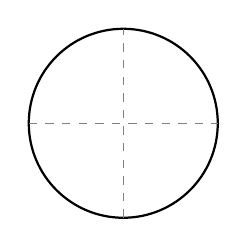
\begin{tikzpicture}[scale=1]
      \draw[thick] (0,0) circle (1.2cm);
      \draw[dashed,gray] (-1.2,0) -- (1.2,0);
      \draw[dashed,gray] (0,-1.2) -- (0,1.2);
    \end{tikzpicture} &
    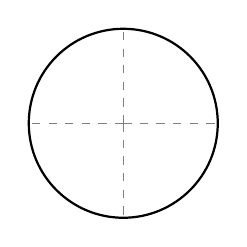
\begin{tikzpicture}[scale=1]
      \draw[thick] (0,0) circle (1.2cm);
      \draw[dashed,gray] (0,0) -- (1.2,0);
      \draw[dashed,gray] (0,0) -- (0,1.2);
      \draw[dashed,gray] (0,0) -- (-1.2,0);
      \draw[dashed,gray] (0,0) -- (0,-1.2);
    \end{tikzpicture} &
    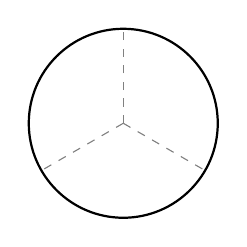
\begin{tikzpicture}[scale=1]
      \draw[thick] (0,0) circle (1.2cm);
      \foreach \a in {90,210,330}
      \draw[dashed,gray] (0,0) -- (\a:1.2);
    \end{tikzpicture} &
    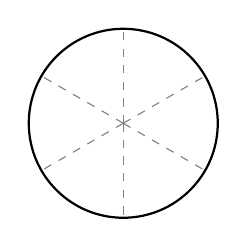
\begin{tikzpicture}[scale=1]
      \draw[thick] (0,0) circle (1.2cm);
      \foreach \a in {30,90,150,210,270,330}
      \draw[dashed,gray] (0,0) -- (\a:1.2);
    \end{tikzpicture}
  \end{tabular}

  \vspace{1cm}

  \item \textbf{Male den angegebenen Bruchteil aus:}
  \begin{enumerate}[label=\alph*)]
    \item Male $\dfrac{3}{8}$ von 8 Kästchen aus: 
    \begin{tabular}{|c|c|c|c|c|c|c|c|}
      \hline
      \phantom{X} & \phantom{X} & \phantom{X} & \phantom{X} & \phantom{X} & \phantom{X} & \phantom{X} & \phantom{X} \\
      \hline
    \end{tabular}

    \vspace{0.3cm}
    \item Male $\dfrac{2}{5}$ von 10 Kreisen aus: $\bigcirc$ $\bigcirc$ $\bigcirc$ $\bigcirc$ $\bigcirc$ $\bigcirc$ $\bigcirc$ $\bigcirc$ $\bigcirc$ $\bigcirc$

    \vspace{0.3cm}
    \item Umkreise $\dfrac{4}{6}$ von 12 Sternen: $\bigstar$ $\bigstar$ $\bigstar$ $\bigstar$ $\bigstar$ $\bigstar$ $\bigstar$ $\bigstar$ $\bigstar$ $\bigstar$ $\bigstar$ $\bigstar$
  \end{enumerate}

  \vspace{0.5cm}

  \item \textbf{Schreibe folgendes als Bruch}
  \begin{enumerate}[label=\alph*)]
    \item Von 10 Äpfeln sind 3 rot: \underline{\hspace{3cm}}
    \item Von 8 Bonbons sind 5 gegessen: \underline{\hspace{3cm}}
    \item Von 12 Monaten sind 4 Sommermonate: \underline{\hspace{3cm}}
  \end{enumerate}
\end{enumerate}